\chapter{Sperimentazione e analisi dei risultati}

I test implementati simulano tre possibili scenari di attacco da parte di uno o più attori malevoli presenti all'interno della rete: \textit{DoS} di \textit{filtering}, l'attacco al $51\%$ ed un comportamento di \textit{selfish mining}.\newline
I dati dei vari test sono stati raccolti eseguendo diverse run per ciascun test utilizzando parametri ad-hoc per i singoli scenari. Con l'ausilio di diversi script in Bash e Python3 è stato possibile aggregare i dati e semplificarli al fine di creare alcuni grafici rappresentativi per una visione ad alto livello dei risultati. I log di ogni singola run sono stati categorizzati in base ai parametri per la successiva fase di aggregazione automatica. Tutti i valori relativi al tempo riportati durante la raccolta dati fanno riferimento al tempo simulato, sono, ovvero, il numero di step eseguiti dal simulatore.
Tutti i test sono stati eseguiti su sistema operativo GNU/Linux ed i grafici sono stati creati utilizzando la libreria Python \href{https://matplotlib.org/}{\texttt{matplotlib}}.\newline
\begin{figure}
    \centering
    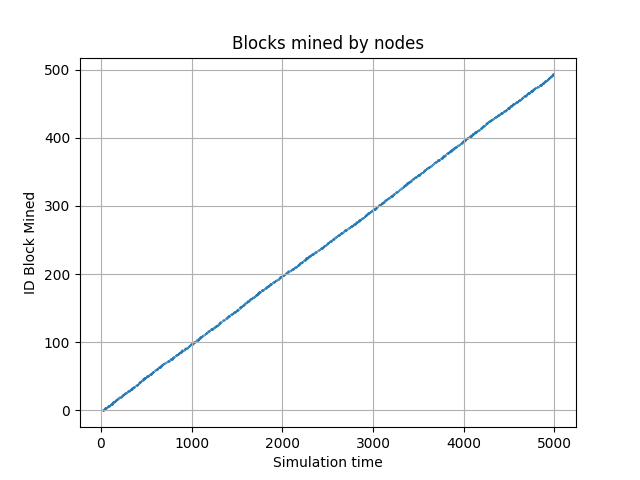
\includegraphics[width=0.8\textwidth]{./images/all-test-51-1.png}
    \caption{Grafico dei blocchi calcolati e diffusi in una rete priva di attaccanti (numero di nodi: $10000$).}
\end{figure}
Utilizzando un \textit{Logical Process} (single-core) una esecuzione di $5000$ step e $10000$ nodi, priva di parametri per la simulazione di scenari di attacco, impiega circa $60s$ per terminare (\textit{Intel i7-6700} con clock \textit{3.40GHz}).\newline
I parametri utilizzati dalla rete e dal protocollo sono raccolti in Tabella~\ref{tab:parameters}.
\begin{table}[H]
    \resizebox{\textwidth}{!}{\begin{tabular}{|l|l|l|}
        \hline
        \begin{tabular}[c]{@{}c@{}}Nome\end{tabular} &
        \begin{tabular}[c]{@{}c@{}}Valore\end{tabular} &
        \begin{tabular}[c]{@{}c@{}}Descrizione\end{tabular} &
        \hline
        \texttt{TTL}                   & 16                   & \textit{Time-To-Live} utilizzato per ridurre l'overhead \\
        \texttt{DISSEMINATION}         & 7                    & Protocollo di disseminazione dipendente dal grado \\
        \texttt{PROBABILITY\_FUNCTION} & 2                    & Funzione dipendente dal grafo con scala logaritmica\\
        \texttt{FUNC\_COEFF\_HIGHER}   & 4                    & Parametro più significativo per la funzione\\
                                       &                      & di propagazione dipendente dal grado\\
        \texttt{FUNC\_COEFF\_LOWER}    & 74                   & Parametro meno significativo per la funzione\\
                                       &                      & di propagazione dipendente dal grado\\
        \texttt{END\_CLOCK}            & 5000                 & Numero di step da eseguire \\
        \texttt{MINERS\_COUNT}         & 70                   & Percentuale dei \textit{miner} rispetto al totale dei nodi\\
        \texttt{DIFFICULTY}            & 6489747252517        & Valore della difficoltà della rete \\
        \texttt{HASHRATE}              & 43983561622000000000 & Totale hashrate della rete espresso in \textit{H/s}\\
        \hline
    \end{tabular}}
    \caption{Tabella parametri utilizzati durante le simulazioni.}
    \label{tab:parameters}
\end{table}

\section{DoS}
Il test realizzato va ad analizzare uno scenario in cui uno o più nodi della rete agiscono come dei ``filtri''; una volta individuata una vittima i messaggi da essa generati non vengono inoltrati nella rete se ricevuti da un nodo attaccante.\newline
Questa tipologia di attacco si evolve in un \textit{Sybil Attack} una volta che tutti i nodi malevoli formano un intorno del nodo vittima.\newline
Il test è stato progettato in modo tale che i nodi attaccanti blocchino ogni tipologia di messaggio creata dal nodo vittima. Questo comporta una possibile mancanza di riconoscimento del lavoro di mining e di validazione o pubblicazione delle transazioni.\newline
I test sono stati eseguiti impostando il numero di nodi attaccanti in maniera incrementale per ogni run. Partendo da una rete in cui è presente un solo nodo attaccante fino al massimo di $9999$. Il test colleziona i dati riguardanti sia i blocchi generati e propagati sia le transazioni create e diffuse in rete.\newline
La raccolta dei dati prevede, per ogni messaggio generato dal nodo vittima, il conteggio dei nodi, in media, che hanno ricevuto il messaggio. Per ciascuna esecuzione è anche possibile utilizzare i log di output per calcolare e visualizzare il numero di nodi raggiunti da ciascun messaggio distinto per \texttt{BlockMsg}, \texttt{TransMsg} o \texttt{AskMsg}.\newline
I risultati ottenuti (Figura:~\ref{fig:dos} e Figura:~\ref{fig:dosmix}) sono compatibili con quelli teoricamente aspettati. Il numero di nodi raggiunti in media dai messaggi del nodo vittima decresce proporzionalmente al numero di attaccanti presenti.\newline
\begin{figure}
    \centering
    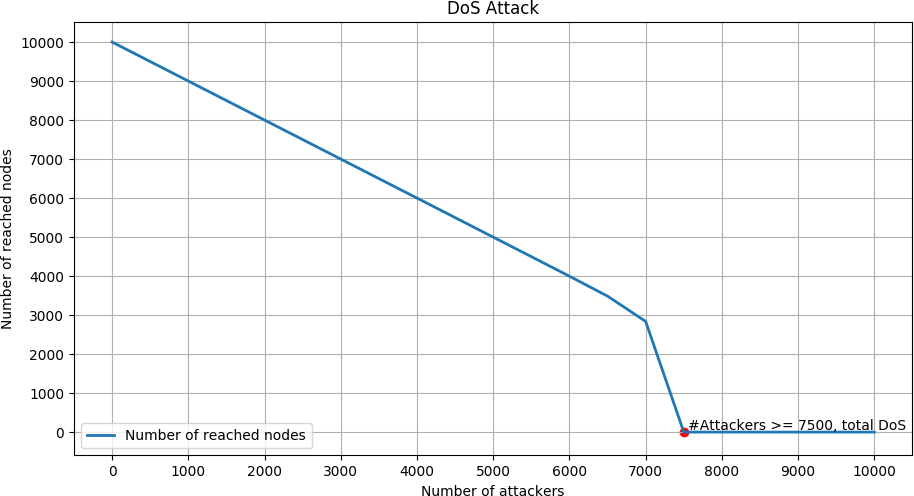
\includegraphics[width=\textwidth]{./images/attackDOS.png}
    \caption{Grafico della media dei nodi raggiunti nelle varie run di test di un attacco \textit{DoS} di tipo \textit{filtering}.}
    \label{fig:dos}
\end{figure}
\begin{figure}[H]
    \centering
    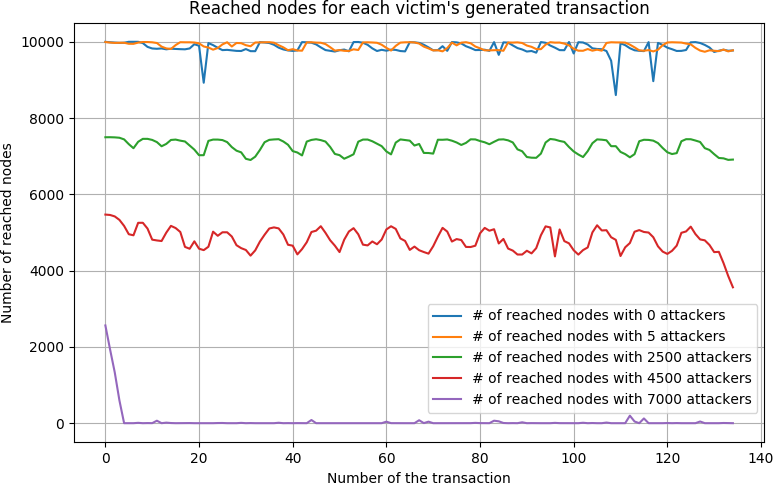
\includegraphics[width=\textwidth]{./images/DOS-mix.png}
    \caption{Confronto del numero di nodi raggiunti per ogni transazione prodotta dal nodo vittima in presenza di diversi numeri di attori malevoli nel caso di \textit{DoS} di tipo \textit{filtering}.}
    \label{fig:dosmix}
\end{figure}
Il numero dei nodi raggiunti si azzera e l'attacco ha completamente successo quando il numero degli attaccanti è tale da escludere il nodo vittima dal resto della rete.\newline
È significativo notare, quindi, che la posizione di un nodo e il numero dei peer vicini (\textit{grado}) sono un elemento fondamentale sulla riuscita o il fallimento dell'attacco. Anche nel caso in cui un solo nodo, non controllato dall'attaccante, propagasse il traffico in uscita dal nodo vittima la rete potrebbe essere ugualmente aggiornata. Nel caso in cui infatti ci sia un solo nodo malevolo tutta la rete, ed esclusione del nodo vittima e attaccante, riceve il messaggio.\newline
È importante sottolineare che nel protocollo \textit{peer-2-peer} i dati scambiati non sono cifrati ma per un nodo malevolo risulta impossibile cambiare questi dati a proprio vantaggio. Anche intercettando un messaggio di pubblicazione di un nuovo nodo, la transazione \textit{coinbase} inserita nel blocco risulta essere valida esclusivamente per il reale proprietario della coppia di chiavi utilizzate per generare la signature. Nel caso in cui un nodo malevolo invalidi un blocco od un messaggio sia ha lo stesso risultato del \textit{DoS} di tipo \textit{filtering} appena presentato.\newline
Al fine di testare anche l'utilizzo dei vari algoritmi di propagazione dei messaggi sono state effettuate ulteriori esecuzioni impostando un \texttt{TTL} maggiore ($20$) e l'algoritmo di propagazione \textit{broadcast} (\texttt{DISSEMINATION=0}). Queste configurazioni generano un elevato overhead nella rete, aumentando i tempo di esecuzione. I risultati ottenuti con questa configurazione sono identici a quelli ottenuti in precedenza in quanto l'algoritmo di propagazione dipendente dal grado ed il \texttt{TTL} impostato in precedenza sono sufficienti a coprire l'intera rete senza un aumento di overhead.\newline
Dati i risultati ottenuti per il testi di \textit{DoS} è possibile affermare la possibilità di successo di un attacco simile è molto bassa. Un attaccante, per poter, controllare il traffico tra i \textit{peer}, deve essere in possesso di numero molto elevato di nodi; questo risulta essere sia infattibile che sconveniente. Nel caso in cui un attaccante controllasse $1000$ nodi risulterebbe più conveniente agire onestamente cercando di sfruttare la potenza di calcolo per ottenere il \textit{reward} tramite mining o abbandonare l'utilizzo dei nodi come accesso alla blockchain ed utilizzarli come una \textit{botnet} per eseguire altri attacchi.\newline

\clearpage
\section{51\% Attack}
L'attacco al $51\%$ apre molteplici scenari in cui uno o più \textit{miner}, in possesso della maggior parte dell'hashrate totale, contribuiscono in maniera esclusiva all'aggiunta dei blocchi nella blockchain primaria. Controllando quali blocchi sono aggiunti alla blockchain un attaccante è in grado di bloccare la conferma delle transazioni e quindi di pagamenti tra utenti e poter effettuare un \textit{double spending}.\newline
Con questo test si vuole osservare come all'aumentare della potenza di \textit{mining} un attaccante possa prendere il sopravvento sull'intera rete.\newline
I test sono stati strutturati variando il numero di \textit{miner}, l'hashrate della rete e quello di un nodo attaccante. Prendendo singolarmente il nodo attaccante è possibile osservare l'andamento dei lavoro di \textit{mining}: l'attaccante ha successo quando il blocco da lui pubblicato raggiunge la maggior parte dei nodi. In questo caso non si è interessati al numero di transazioni create, ricevute od inserite nella blockchain ma solo al numero di blocchi trovati; per questo al fine di aumentare le performance e ridurre i tempo di esecuzione sono state disabilitate queste funzionalità.
\begin{figure}[H]
    \centering
    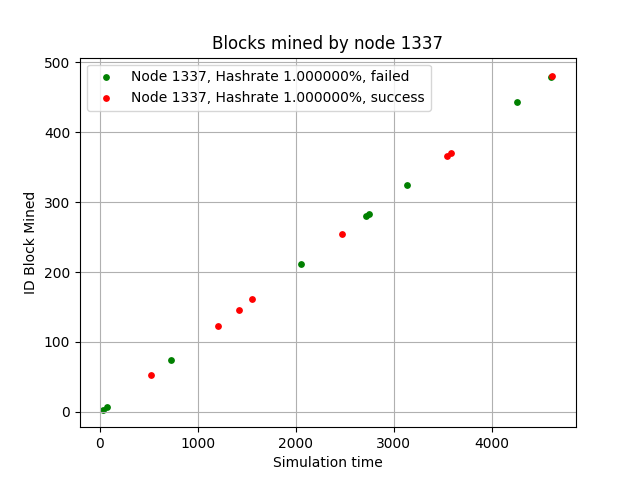
\includegraphics[width=\textwidth]{./images/1337-test-51-1.png}
    \caption{Grafico dei blocchi calcolati e diffusi nella rete dall'attaccante (nodo $1337$) con il $1\%$ dell'hashrate totale.}
    \label{fig:51v1.1}
\end{figure}
\begin{figure}[H]
    \centering
    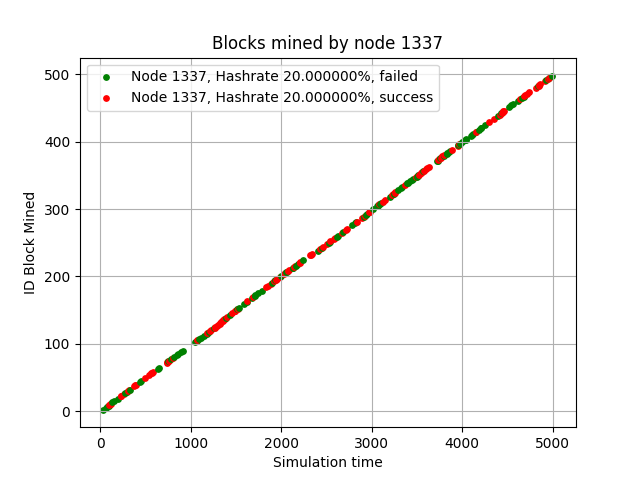
\includegraphics[width=\textwidth]{./images/1337-test-51-20.png}
    \caption{Grafico dei blocchi calcolati e diffusi nella rete dall'attaccante (nodo $1337$) con il $20\%$ dell'hashrate totale.}
    \label{fig:51v1.20}
\end{figure}
Una prima versione dell'attacco è stata eseguita configurando la rete con i parametri della Tabella~\ref{tab:parameters} e la potenza di calcolo dell'attaccante crescente dall'$1\%$ al $100\%$.
Come è possibile vedere dalle due immagini precedenti (Figura~\ref{fig:51v1.1} e Figura~\ref{fig:51v1.20}) all'aumentare dell'hashrate dell'attaccante aumenta anche il numero di nodi prodotti ma ciò non garantisce che i nodi vengano accettati da tutti i nodi in quanto gli altri \textit{miner} potrebbero aver pubblicato il blocco prima o aver raggiunto la maggior parte dei nodi in minor tempo.\newline
Elaborando tutti i dati delle esecuzioni è possibile visualizzare l'andamento tra hashrate e percentuale di successo dell'attaccante (Figura~\ref{fig:51v1}).
\begin{figure}[H]
    \centering
    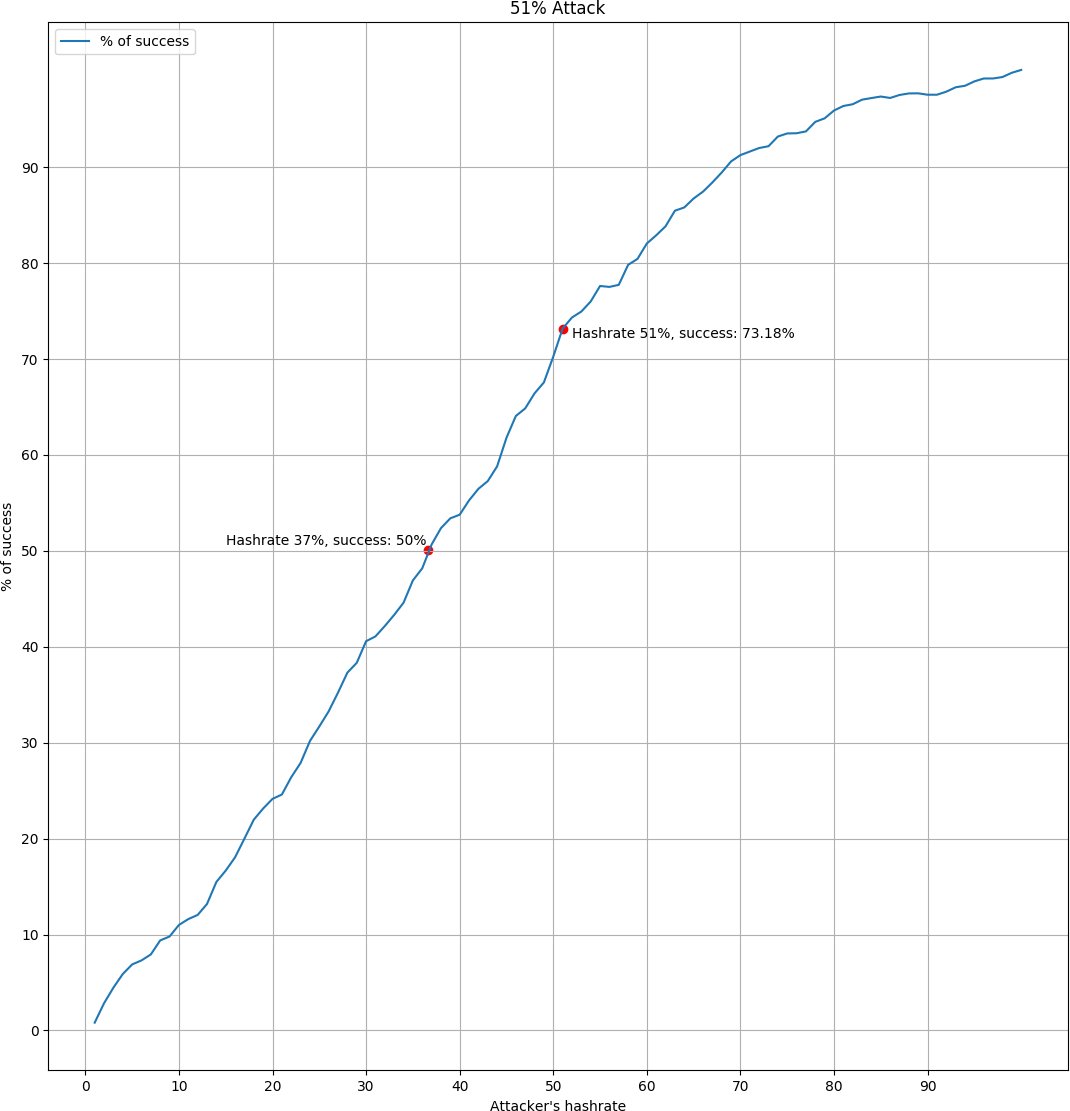
\includegraphics[width=\textwidth]{./images/51-v1.png}
    \caption{Attacco del $51\%$, versione 1.}
    \label{fig:51v1}
\end{figure}
Sorprendentemente le percentuali di successo sono molto elevate anche per hashrate al di sotto del $51\%$. Per la soglia del $51\%$ sia ha che la possibilità di successo è molto alta ($73.18\%$); la facilità dell'attacco rilevata è dovuta ad una errata modellazione del test: il $70\%$ di \textit{miner} della rete è una percentuale troppo elevata e questo comporta un hashrate per nodo estremamente basso. La media dell'hashrate per i nodi è dello $0.0142\%$; tale configurazione aumenta notevolmente le possibilità di successo per l'attaccante in quanto non esistono dei \textit{miner} capaci di contrastare una potenza di calcolo molto alta. Anche solo l'$1\%$ risulta essere $70$ volte superiore alla media.\newline
Un secondo tentativo (Figura~\ref{fig:51v2}) è stato effettuato riducendo al $20\%$ il numero di miner.
\begin{figure}[H]
    \centering
    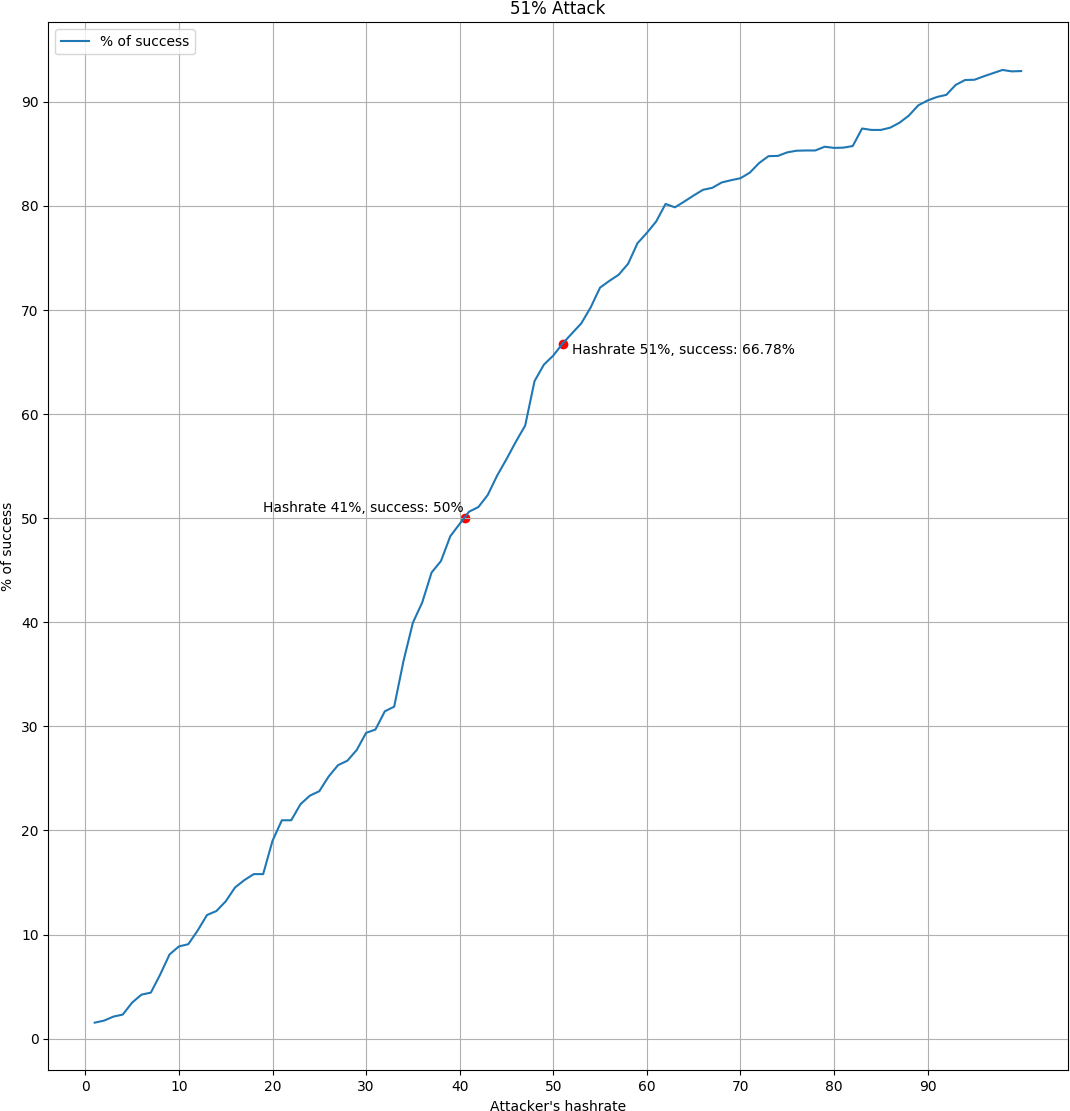
\includegraphics[width=\textwidth]{./images/51-v2.png}
    \caption{Attacco del $51\%$, versione 2.}
    \label{fig:51v2}
\end{figure}
Anche in questo caso i risultati sono a favore dell'attaccante ma la riduzione dei \textit{miner} ha incrementato la media dell'hashrate per ogni nodo contrastando, in minima parte, l'attività dell'attaccante.\newline
Infine, è stato eseguito un test con $15$ \textit{miner} ed un ulteriore miglioramento: l'hashrate dell'attaccante non è calcolato in percentuale all'intera rete ma viene sommato al totale. L'hashrate totale della rete con un attaccante con una potenza di calcolo del $20\%$, ad esempio, è del $120\%$. In un caso reale l'attaccante deve inserirsi nella rete con il massimo della potenza che dispone al fine di evitare sia una riorganizzazione della rete e della community sia un aumento della difficoltà dovuta all'aumento dell'hashrate.\newline
Riducendo quindi sia numero di \textit{miner} totali e strategia dell'attaccante è possibile vedere (Figura~\ref{fig:51v3}) come effettivamente la soglia del $51\%$ garantisca all'attaccante un successo di poco superiore al $50\%$. Una riflessione va fatta anche per il caso in cui l'attaccante abbia il $100\%$ della potenza di calcolo; data l'alta varianza della funzione di probabilità non si ha la certezza assoluta che il blocco venga calcolato dal \textit{miner} con il più alto \textit{hashrate}.
\begin{figure}[H]
    \centering
    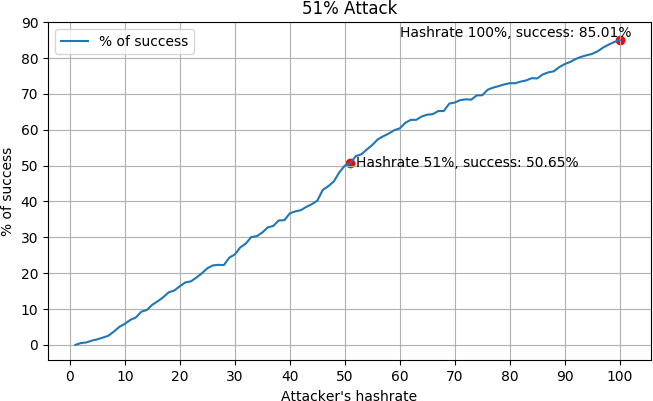
\includegraphics[width=\textwidth]{./images/51-v3.png}
    \caption{Attacco del $51\%$, versione 3.}
    \label{fig:51v3}
\end{figure}
Questo attacco deve essere visto come un gradiente e non come una soglia in quanto anche con soglie di hashrate minori del $51\%$ le probabilità di successo non sono trascurabili. Con gli attuali valori di hashrate (Novembre 2018) il costo per ottenere il $51\%$ di potenza per un'ora tramite cloud computing è di $14~682~645$\$\footnote{\href{https://www.crypto51.app/}{crypto51.app}}. In un'ora vengono pubblicati circa $10$ blocchi per un possibile \textit{reward} totale di $125$ BTC, ovvero $793~625$\$, che potrebbe essere utilizzato per ammortizzare il costo iniziale. Nonostante la possibilità di guadagno ottenuti dai \textit{reward} e da eventuali \textit{double spending} effettuati in un'ora di tempo, è altamente improbabile che qualcuno investa la cifra di $13~889~020$\$ per ottenere poco più del $50\%$ di possibilità di successo.\newline
Un attacco del $51\%$ non è mai stato registrato per la blockchain Bitcoin con il fine di essere sfruttato per scopi malevoli ma nel 2014 l'hashrate del \textit{pool} \textit{Ghash.IO} raggiunse questa soglia. La community, presa visione della possibile problematica, discusse su come trovare una soluzione; il \textit{pool}, volontariamente, decise di ridurre la propria potenza di calcolo. Bitcoin, data la sua vasta adozione ed una community molto numerosa, potrebbe non essere mai affetto da questa problematica ma altre criptomonete come \textit{MonaCoin}, \textit{Bitcoin Gold} (una \textit{fork} di Bitcoin), \textit{ZenCash}, \textit{LiteCoin} ed altre minori sono state sfruttate per operare questo attacco. In questi casi si è trattato di veri e propri attacchi in cui gli attori malevoli sono riusciti a dirottare l'evoluzione della catena a proprio favore. Nell'attacco apportato a \textit{ZenCash} gli attaccanti hanno sfruttato la loro potenza di calcolo per creare delle transazioni a proprio vantaggio per un totale di $21000$ token ($\sim50000$\$). Per ottenere un hashrate pari al $109\%$ sulla rete per \textit{MonaCoin} sono sufficienti $624$\$ (contro i $277536$\$ per l'$1\%$ su rete Bitcoin, dati aggiornati a Novembre 2018).

\section{Selfish Mining}
Il test realizzato va ad analizzare uno scenario in cui un \textit{miner} implementa una strategia di \textit{selfish mining} al fine di ottenere maggiori guadagni derivati dalla attività di \textit{mining}.\newline
L'implementazione è quella proposta dal paper~\cite{selfish} \textit{``Majority is not Enough: Bitcoin Mining is Vulnerable''} e descritta in \ref{lst:selfish}. Utilizzando una struttura dati per salvare lo stato della blockchain privata e pubblica è stato possibile realizzare uno scenario in cui un attaccante, con crescente hashrate, applica un strategia di \textit{selfish mining}.\newline
L'attaccante aggiunge alla propria blockchain privata il blocco $b$ senza propagarlo nella rete. Una volta che è riuscito a calcolare il blocco $b+1$ o ha ricevuto da un altro nodo il blocco $b$, pubblica i blocchi trovati in precedenza. In questo modo nella rete si crea una condizione di \textit{race condition} tra il nodo $b$ dell'attaccante e quello generato dai nodi onesti.\newline
L'attaccante quindi accumula più blocchi possibile prima di pubblicarli (in questo caso $2$), l'attacco ha successo se riesce ad accumulare almeno due blocchi consecutivi senza che la rete ne abbia ancora divulgato uno e la maggior parte dei \textit{peer} lo accetta nella propria blockchain.\newline
La strategia proposta da \textit{Eyal} e \textit{Sirer}~\cite{selfish} garantisce che con un hashrate relativamente basso ($\sim33\%$) una simile strategia può incrementare i guadagni nel breve termine derivanti dal \textit{mining}. L'attacco è stato studiato per essere applicato ai \textit{mining pool} che, se dovesse applicare questa strategia, potrebbe essere utilizzato da più \textit{miner} riducendo la possibilità di successo degli altri e rendendo la rete sempre meno decentralizzata.
\clearpage
\begin{code}
    \captionof{listing}{Comportamento del \textit{selfish miner} durante la fase di \textit{mining}.}
\begin{minted}[breaklines]{c}
// If the attack is enabled
if (node->data->attackerid == node->data->key && selfish[2] >= 0) {
    // clock - nodeid - blockminedid - hashrate (BSS is a debug tag)
    fprintf(stdout, "BSS: %.0f,%d,%d,%f\n", simclock, node->data->key, ltblock, node->data->hashrate);
    // Status
    selfish[2] += 1;
    // Private blockchain
    selfish[0]  = ltblock;
    // if the attacker has mined two blocks the attacks is sucessful, broadcast all
    if (selfish[2] >= 2) {
        // Debug print
        fprintf(stdout, "possible selfish successful %d %d %d\n", selfish[0], selfish[1], selfish[2]);
        // Send the two found blocks
        lunes_send_block_to_neighbors(node, &node->data->s_state.blockchain[ltblock - 1]);
        lunes_send_block_to_neighbors(node, &node->data->s_state.blockchain[ltblock]);
        selfish[2] = 0
    }
}
\end{minted}
\end{code}
Il comportamento alla ricezione di un blocco è modellato nella routine di gestione dei messaggi \texttt{BlockMsg}. Se l'attaccante riceve il blocco $b$, presente come ultimo nella blockchain privata, allora l'attacco è fallito. Se invece riceve un blocco più obsoleto divulga i blocchi non ancora pubblicati.
\clearpage
\begin{code}
    \captionof{listing}{Comportamento del nodo attaccante durante una ricezione di un messaggio \texttt{BlockMsg} secondo il modello proposto in \ref{lst:selfish}.}
\begin{minted}[breaklines]{c}
int ltblock         = node->data->latestblock;
int receivedblockid = msg->block.block_static.minedblock->id;
// If the attacker receive a block present in his private blockchain
// publish only the needed blocks
// selfish[2] = number of mined block in private's blockchain
if (node->data->attackerid == node->data->key && selfish[2] >= 0) {
    int diff_prev = selfish[0] - receivedblockid;
    // Update the status of the public blockchain
    selfish[1] = receivedblockid;
    if (diff_prev == 0) {
        // Reset the counter
        selfish[0] = receivedblockid
        selfish[2] = 0;
    }else if (diff_prev == 1) {
        // Send the last mined block in the private blockchain
        lunes_send_block_to_neighbors(node, &node->data->s_state.blockchain[selfish[0]]);
    }else if (diff_prev == 2) {
        // Clear the buffer: send all blocks
        // for each privately mined block send it
        for (int b = selfish[0]; b >= 0; --b) {
            // Broadcasting the mined old blocks to all neighbors
            lunes_send_block_to_neighbors(node, &node->data->s_state.blockchain[selfish[0] - b]);
        }
        selfish[2] = 0;
    }else {
        // Send first unpublished block from private chain
        int first_unp_block = selfish[0] - selfish[2] - 1;
        lunes_send_block_to_neighbors(node, &node->data->s_state.blockchain[first_unp_block]);
    }
}
\end{minted}
\end{code}
Come per l'attacco del $51\%$ il test ha successo se la maggior parte dei nodi ricevono uno o più blocchi pubblicati dall'attaccante durante la fase di divulgazione della blockchain privata.\newline
È possibile considerate un successo sia se un singolo blocco della blockchain privata ha raggiunto la maggior parte dei nodi sia se una coppia di blocchi consecutivi è stata aggiunta alla blockchain pubblica. Questo ultimo caso garantisce all'attaccante il massimo del guadagno previsto e rende inutile il lavoro effettuato dagli altri \textit{miner} in quanto vengono pubblicati due blocchi nella rete che non sono ancora stati aggiunti alla blockchain pubblica.\newline
Questa strategia comporta il rischio di non aver nessun guadagno dal lavoro di \textit{mining} se gli altri \textit{peer} della rete pubblicano ed accettano un blocco prima che quello dell'attaccante sia stato divulgato (rendendolo orfano).
\begin{figure}[H]
    \centering
    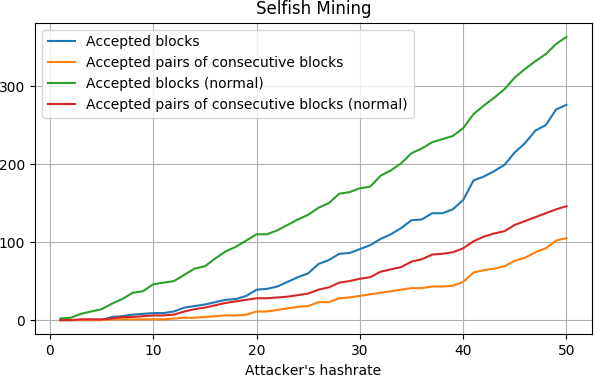
\includegraphics[width=\textwidth]{./images/selfishtest.png}
    \caption{Visualizzazione dei dati ottenuti dal test di \textit{selfish mining}. Il grafico conteggia sia il numero dei singoli blocchi accettati sia le coppie di blocchi entrate nella blockchain pubblica per una strategia di mining normale e uno di \textit{selfish mining}.}
    \label{fig:selfishtest}
\end{figure}
Dai dati ricavati dai test (Figura ~\ref{fig:selfishtest}) è possibile osservare che la strategia di \textit{selfish mining} (linea blu ed arancio) non comporta vantaggi in quanto sia il numero di blocchi, sia il numero di coppie di blocchi consecutivi sono minori di quelli rilevati non applicando una strategia (linea verde e rossa). Questa discrepanza tra i dati rilevati e quelli proposti dal paper è dovuta al fatto che i risultati dello studio si basano solo su calcoli matematici tramite l'utilizzo di distribuzioni di probabilità di eventi indipendenti\footnote{Due eventi si definiscono indipendenti se l'occorrenza di uno non influenza la probabilità che si verifichi il secondo.} e prende in considerazione anche eventuali ritardi dovuti alla latenza di rete o dei client. Queste distribuzioni sono utili nel caso in cui non ci siano eventi correlati ma nel caso del \textit{selfish mining} è da notare che la diffusione dei blocchi della blockchain privata dipendono dall'evento di ricezione di un blocco per decidere la strategia da adottare al passo successivo. È stato infatti discusso~\cite{selfishfallacy} che la strategia di \textit{selfish mining} non garantisce sempre maggiori guadagni ma rallenta la frequenza con cui i blocchi vengono inseriti nella blockchain; di conseguenza in un lasso di tempo ben definito è possibile che il numero di blocchi pubblicati nella rete sia inferiore. L'aumento del tempo di \textit{mining} tra i blocchi comporta una diminuzione delle ricompense dovute al \textit{mining} rispetto a quelle previste con una frequenza maggiore.\newline
Il paper che ha proposto questa strategia non è da considerarsi errato o fuorviante in quanto la strategia prevede anche che i \textit{miner} onesti si aggreghino al \textit{selfish miner} e che la rete, dato il ritardo nella propagazione dei blocchi, aggiusti la \textit{difficoltà} ad un valore più basso (avvantaggiando l'attaccante). I dati ottenuti rappresentano una casistica della strategia in cui non ci sono ritardi di rete, cambiamenti da parte degli altri miner e aggiustamenti del valore di \textit{difficoltà}.\newline


% NeoTex: mainfile=main.tex:
